%% Revisado por Gabriel Saraiva

\chapter{Testes, resultados e avaliações}
\label{cap4}

Nesse capítulo serão apresentados os ambientes de testes e os resultados obtidos.

\section{Ambiente de Testes}

    O ambiente de testes utilizou os equipamentos disponíveis no laboratório do GSPD e um celular próprio.
    
    Esses equipamentos são:
    
    \begin{itemize}
    
    \item \textit{Cluster} heterogêneo com 16 nós:
    
        \begin{itemize}
        \item 8 nós equipados Intel(R) Core(TM) i7, 16GB de RAM, HD de 500GB
        \item 8 nós com Intel(R) Pentium(R) Dual, 4 GB de RAM, HD de 80GB
        \item Conexão 10/100/1000
        \end{itemize}
        
    \item \textit{Tablet} Samsung GALAXY Note 10.1 - 2014 (referente ao processo FAPESP 2012/02926-5):
        
        \begin{itemize}
            \item Android 4.3 (Jelly Bean)
            \item 3 GB de memória RAM
            \item 16GB de armazenamento interno (\textit{flash})
            \item bateria de 8220 mAh
            \item Chipset Qualcomm Snapdragon 800
            \item CPU Quad-core 1.9 GHz Cortex-A15
            \item GPU Adreno 330
        \end{itemize}
        
    \item \textit{Smart-phone} Motorola Moto X XT1058:
    
        \begin{itemize}
            \item Android  4.4.4 (KitKat)
            \item 2GB de memória RAM
            \item 16GB de armazenamento interno (\textit{flash})
            \item bateria de 2200 mAh
            \item Chipset Qualcomm MSM8960DT Snapdragon S4 Pro
            \item CPU Dual-core 1.7 GHz Krait 300
            \item GPU Adreno 320
            
        \end{itemize}
        
    \item Roteador Wi-fi Asus 300 Mbps
    
    \end{itemize}
    
     Nos testes de desempenho e eficiência, para amenizar influências de outros processos e do sistema operacional, os testes foram realizados 10 vezes com intervalos aleatórios de 1 a 2 minutos. Os tempos utilizados nos gráficos são as médias dessas execuções. Além disso, também foram calculados os desvios padrões.

\section{Integridade dos Dados}

Como segundo ~\cite{coulouris}, um dos principais deveres de um sistema de arquivos distribuídos é manter a integridade de seus arquivos, foram feitos testes de integridade dos arquivos, para verificar se o processo de criptografia e transmissão dos arquivos não danificaram os arquivos. Esses testes foram feitos com arquivos de 100KB, 5MB e 200MB.
    
    Inicialmente era calculado o \textit{hash} MD5 dos arquivos, que então eram copiados via cabo de dados para os dispositivos móveis. Então eram transferido e recuperados do FlexA via Wi-fi, e então eram novamente copiados para um computador via cabo de dados. Depois era calculado o \textit{hash} MD5 dos arquivos para mostrar a integridade dos mesmos. A figura \ref{fig:testesIntegridade} mostra os resultados.

    \begin{figure}[!ht]
    \centering
    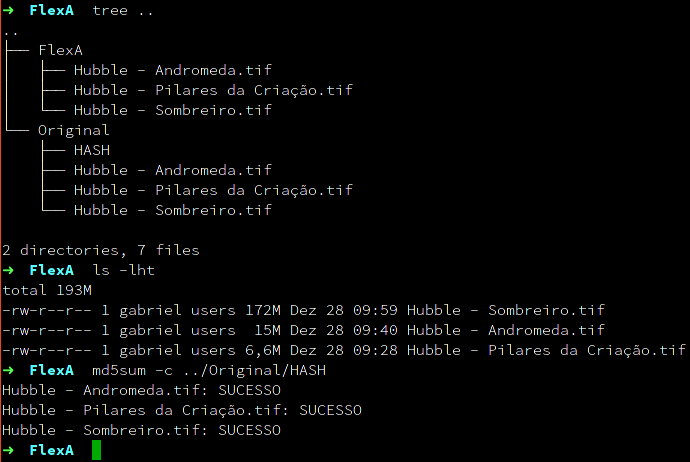
\includegraphics[width=14cm]{testeIntegridade.png}
    \caption{Teste de integridade dos arquivos. Nenhum arquivo foi danificado durante os testes.}
    \label{fig:testesIntegridade}
    \end{figure}

    Todos os testes mostraram resultados positivos quanto a integridade dos arquivos ao serem enviados e retornarem pelo FlexA.
    
\section{Compatibilidade do sistema}

    Como o módulo cliente implementado do FlexA deve ser compatível com o módulo existente, foram feitos testes semelhantes aos de integridade mostrado anteriormente, exceto que os arquivos eram inseridos no FlexA pelo cliente em Python e depois recuperados pelo cliente Android e vice e versa. Na figura \ref{fig:testeCompatibilidade} são apresentados os resultados desse teste.
    
    \begin{figure}[!ht]
    \centering
    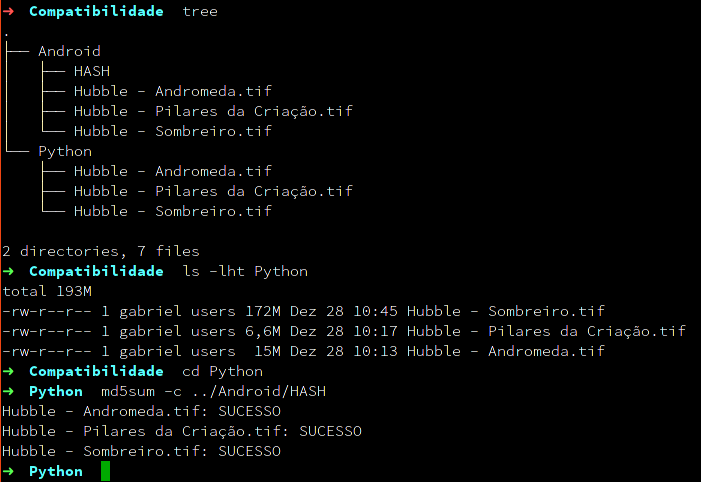
\includegraphics[width=14cm]{testeCompatibilidade.png}
    \caption{Teste de compatibilidade entre os dois módulos clientes do FlexA. Nenhum arquivo foi danificado durante os testes mostrando que os sistemas estão compatíveis.}
    \label{fig:testeCompatibilidade}
    \end{figure}
    
\section{Desempenho de criptografia}

    Esse teste mostra o tempo necessário para criptografar arquivos com 100KB, 5MB e 200MB em cada um dos dispositivos móveis e também em um nó do primeiro grupo do \textit{cluster} (computadores com processador Intel Core i7) para comparação. Os resultados são mostrados na figura \ref{fig:testesCriptografia}.
    
    \begin{figure}[!ht]
    \centering
    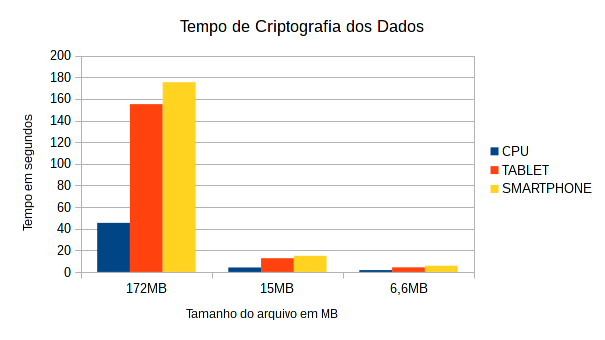
\includegraphics[width=14cm]{testeCriptografia.png}
    \caption{Teste de desempenho de criptografia com clientes diferentes do FlexA}
    \label{fig:testesCriptografia}
    \end{figure}
    
    Como esperado o computador do \textit{cluster} foi capaz de criptografar os arquivos aproximadamente 10 vezes mais rápido que o \textit{tablet} e 11 vezes mais rápido que o \textit{smart-phone}.
    
\section{Desempenho de transmissão dos dados}

    Esse teste mostra o tempo necessário para enviar e receber arquivos com 100KB, 5MB e 200MB em cada um dos dispositivos móveis e também em um nó do primeiro grupo do \textit{cluster} (computadores com processador Intel Core i7) para comparação. Os resultados são mostrados na figura \ref{fig:testeTransmissao}.
    
    \begin{figure}[!ht]
    \centering
    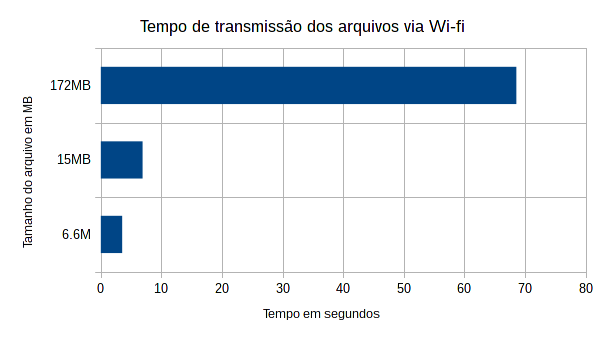
\includegraphics[width=14cm]{testeTransmissao.png}
    \caption{Teste de desempenho de transmissão de arquivos com clientes diferentes do FlexA}
    \label{fig:testeTransmissao}
    \end{figure}
    
    Como esperado o computador do cluster foi capaz de enviar e receber os arquivos aproximadamente 20 vezes mais rápido que o \textit{tablet} e o \textit{smart-phone}, já que está conectado aos servidores do FlexA via rede \textit{gigabit}. Os resultados das transmissões dos dispositivos móveis mostra que embora existam três servidores o ganho de desempenho por utilizá-los é insignificante, pois o gargalo nesse caso é a transmissão sem fio dos dados.